% ==================================================================
%---------BLOQUE 1------------------- (Preambulo y datos del documento)
%====================================================================
% INFORME DEL PROYECTO FINAL, CA-0309 CONTINGENCIAS DE VIDA II
% Grupo 2: Auditoría o Control
%
% Compilar con LuaLaTeX, dos veces.
% Las tablas y la figura las genera Codigo/main.R en salidas/
%====================================================================



% !TEX program = lualatex
\documentclass[10pt,a4paper]{article}

% ---------- Matemática y fuentes ----------
\usepackage{amsmath,mathtools}
\usepackage{amsthm}
\usepackage{fontspec}
\usepackage{unicode-math}
\setmathfontface\mathsf{Latin Modern Sans}   % Sans-serif matemático
\setmathfontface\mathtt{Latin Modern Mono}   % Typewriter matemático
\setmathfont{NewCMMath-Book}
% ---------- Idioma ----------
\usepackage{polyglossia}
\setmainlanguage{spanish}
\addto\captionsspanish{%
	\renewcommand{\contentsname}{Tabla de contenidos}%
	\renewcommand{\tablename}{Tabla}%
}
% ---------- Diseño ----------
\usepackage[a4paper,top=1.7cm,bottom=1.7cm,left=1.4cm,right=1.4cm,headsep=0.35cm]{geometry}
\usepackage{tabularx}
\setlength{\emergencystretch}{2.5em} % evita líneas que se salen
\usepackage{microtype}
\usepackage{enumitem}
\usepackage[table]{xcolor}
\usepackage{booktabs}
\usepackage{float} % [H] fija la tabla donde se escribe
\usepackage{fancyhdr}
\setlength{\headheight}{11pt}
\pagestyle{fancy}
\fancyhf{}
\renewcommand{\headrulewidth}{0pt}
\fancyhead[R]{\small\itshape Informe del proyecto final}
\fancyfoot[C]{\small\thepage}

% ---------- Enlaces y referencias cruzadas ----------
\usepackage[colorlinks=true,linkcolor=blue!40!black,citecolor=blue!40!black,urlcolor=blue!40!black]{hyperref}
\usepackage[capitalise]{cleveref}
\usepackage{graphicx}
\usepackage{subcaption}

\crefname{section}{Sección}{Secciones}
\crefname{table}{Tabla}{Tablas}
\crefname{figure}{Figura}{Figuras}
\crefname{equation}{ecuación}{ecuaciones}
\crefname{subsection}{Subsección}{Subsecciones}

% ---------- Numeración ----------
% Las secciones del trabajo común van de A a F, como en la guía.
\renewcommand{\thesection}{\Alph{section}}
\numberwithin{equation}{section}

% ---------- Macros del informe ----------
% Tablas exportadas por R (solo el tabular; aquí se pone el caption)
\newcommand{\tabla}[1]{\input{salidas/tablas/#1.tex}}
\newcommand{\um}{u.m.}

% Texto predeterminado
\newcommand{\ph}[1]{\textcolor{red!70!black}{\textit{[#1]}}}

% ---------- Encabezado a una sola columna (franja centrada) ----------
% \maketitle escribe título, autores, afiliaciones, fecha, resumen y palabras clave
% en una franja centrada de ancho \anchofranja (cámbiese el 0.78 para ensancharla o angostarla).
\newcommand{\anchofranja}{0.78\textwidth}
\makeatletter
\newcommand{\resumen}[1]{\gdef\@resumen{#1}}
\newcommand{\palabrasclave}[1]{\gdef\@palabrasclave{#1}}
\newcommand{\afiliaciones}[1]{\gdef\@afiliaciones{#1}}
\let\@resumen\@empty
\let\@palabrasclave\@empty
\let\@afiliaciones\@empty
\renewcommand{\@maketitle}{%
	\newpage\null\vskip 1em
	\begin{center}
		\begin{minipage}{\anchofranja}
			\centering
			{\Large \@title\par}
			\vskip 1em
			{\def\and{\unskip,\hskip 0.8em plus 0.3em\ignorespaces}\normalsize \@author\par}
			\ifx\@afiliaciones\@empty\else
			\vskip 0.5em
			{\footnotesize \@afiliaciones\par}
			\fi
			\vskip 0.8em
			{\small \@date\par}
			\ifx\@resumen\@empty\else
			\vskip 1.2em
			\begin{minipage}{\linewidth}% texto justificado dentro de la franja
				\noindent{\small\bfseries\abstractname}\par
				\vskip 0.4em
				\small\@resumen\par
				\ifx\@palabrasclave\@empty\else
				\vskip 0.5em
				\noindent\textbf{Palabras clave:} \@palabrasclave\par
				\fi
			\end{minipage}
			\fi
		\end{minipage}
	\end{center}
	\vskip 1em}
\makeatother



%====================================================================
% DATOS DEL DOCUMENTO
%====================================================================
\title{\textbf{Seguro colectivo de fallecimiento y cuenta equity-linked:\\ proyección, profit testing y riesgo a cinco años} \\[0.4em]
	\large Informe del proyecto final \,|\, Grupo 2, Auditoría o Control}

\author{%
	Andrey Gonzales (C33329)\textsuperscript{1} \and
	Randal Picado Bermúdez (C36024)\textsuperscript{1} \and
	Anthonny Flores Rojas (C32975)\textsuperscript{1}}

\afiliaciones{%
	\textsuperscript{1}Escuela de Matemática, Universidad de Costa Rica}

\date{Curso: Contingencias de Vida II (CA-0309) \\
	Profesora: Yerling Ramírez Morera \\[0.3em] \today}

\resumen{%
	Se proyecta a cinco años un seguro colectivo de fallecimiento para los 104\,004 activos del Fondo mutual, con mortalidad de Costa Rica 2023 y renuncia del 3\,\% como decrementos competitivos, y una cuenta equity-linked para un hombre representativo de 45 años. Con los parámetros de la guía, el seguro colectivo tiene un NPV de \(-12\,912.86\) millones de \um\ y un margen de \(-57.88\,\%\): la prima neta de gasto y comisión no cubre el siniestro esperado en ningún año y los recursos no respaldan la reserva suministrada desde el primer cierre. El escenario adverso empeora el resultado y el estrés del grupo 2 (prima de 55\,000 y renuncia del 6\,\%) lo mejora sin volverlo rentable, a costa de 12\,312 asegurados menos. En la cuenta equity-linked, la garantía de 100\,000 domina a la de 110\,000 en NPV medio y en pérdidas de cola. Como Auditoría o Control recomendamos posponer el seguro colectivo y apoyar la cuenta con \(G=100\,000\).}

\palabrasclave{profit testing, decrementos múltiples, varias vidas, equity-linked, NIIF 17.}



%---------BLOQUE 2------------------- (Opinión ejecutiva y supuestos)
\begin{document}

	\maketitle

	\section*{Opinión ejecutiva}\label{sec:opinion}

	Como grupo de Auditoría o Control revisamos la proyección a cinco años del seguro colectivo de fallecimiento y de la cuenta equity-linked que una aseguradora propone para el Fondo mutual. Todos los montos del seguro colectivo están en millones de unidades monetarias (\um) salvo que se indique otra cosa.

	Con los parámetros de la guía, el seguro colectivo no es rentable. El NPV base es de \(-12\,912.86\) millones y el margen sobre primas descontadas es de \(-57.88\,\%\). El problema es de tarifa y no de un supuesto aislado: la prima neta de gasto y comisión (37\,500 por contrato) queda por debajo del siniestro esperado por contrato en los cinco años (de 46\,659 a 57\,392), y el gasto de adquisición explica por sí solo 7\,800.30 millones de la pérdida. Además, los recursos no respaldan la reserva suministrada desde el cierre del año 1 en ninguno de los tres escenarios, y la base necesita 3\,050.20 millones de aportes.

	El escenario adverso (gasto de 11\,000 y rendimiento del 4\,\%) lleva el NPV a \(-13\,617.35\) millones. Nuestro escenario de estrés (prima de 55\,000 y renuncia del 6\,\%) lo mejora a \(-10\,222.77\) millones y elimina los aportes, pero termina con 12\,312 activos menos al cierre del año 5 y el producto sigue perdiendo. En la cuenta equity-linked, la garantía de 100\,000 domina a la de 110\,000 en resultado medio y en cola.

	\begin{center}
		\fbox{\begin{minipage}{0.94\textwidth}
				\textbf{Opinión del grupo 2.} \textit{Posponer} el seguro colectivo hasta contar con una tarifa que dé NPV no negativo en base y adverso, y con un plan de capital que respalde la reserva desde el año 1. \textit{Apoyar} la cuenta equity-linked con \(G=100\,000\) (NPV medio 4\,054.40, frecuencia de pérdida 24.6\,\%, CTE\(_{95}\) 22\,959.79), condicionada a monitorear la cola de pérdidas.
		\end{minipage}}
	\end{center}

	\section*{Datos y supuestos}\label{sec:datos}

	Se usó la hoja \textit{Activos} de la base del Fondo, con edades en años cumplidos al 31/12/2025, y la mortalidad de Costa Rica 2023 por edad y sexo. Los supuestos del producto son los de la guía~\cite{Guia2026}: renuncia de decremento único \(r=3\,\%\), prima \(C=50\,000\), beneficio \(b=5\,000\,000\), gasto \(e=10\,000\) por vigente, comisión \(\alpha=5\,\%\), adquisición \(k=75\,000\) por contrato, recursos iniciales de \(100\,000N_0\), rendimiento \(i=5\,\%\) y descuento \(d=4\,\%\) (factor \(v=1/1.04\)). Prima, gasto y comisión se pagan al inicio del año y los beneficios al cierre. Todo se programó en R (4.5.1) y las tablas se exportan desde el código con \texttt{source("Codigo/main.R")}; ninguna cifra se editó a mano.

	%---------BLOQUE 3------------------- (A: población y decrementos)
	\section{Población, decrementos y multiestado}\label{sec:A}

	\subsection{Base inicial}

	De los 104\,142 registros de Activos se segregaron 138 por la primera causa que cumplían, en el orden de la \cref{tab:registros}, para no contar a nadie dos veces. No hubo identificadores duplicados ni edades fuera de 0 a 106. Ningún identificador de Activos aparece en las hojas Fallecidos (1\,061 registros) o Inactivos (456), así que no fue necesario revisar casos cruzados. La población inicial es \(N_0=104\,004\) (52\,652 mujeres y 51\,352 hombres), con edad media de 51.2 años y rango de 1 a 96. Las cuotas, leídas como \(n/12\) años equivalentes de aportación, van de 0.08 a 23.17 años, con mediana 8.42 y media 9.64; solo se describen y no se usan en ningún cálculo.

	\subsection{Decrementos y matriz de transición}

	Para cada edad \(x\) y sexo, la mortalidad de tabla \(q'^{(d)}_x\) y la renuncia \(q'^{(w)}=0.03\) son probabilidades de decremento único~\cite{Dickson2020}. Con fuerzas constantes dentro del año,
	\begin{equation}\label{eq:decrementos}
		p^{(\tau)}_x=\bigl(1-q'^{(d)}_x\bigr)\bigl(1-q'^{(w)}\bigr),\qquad
		q^{(j)}_x=\frac{\ln\bigl(1-q'^{(j)}_x\bigr)}{\ln p^{(\tau)}_x}\,\bigl(1-p^{(\tau)}_x\bigr),\quad j\in\{d,w\}.
	\end{equation}
	En el año \(t\), la cohorte de edad inicial \(a\) usa la edad \(a+t-1\): \(D_t=N_{t-1}q^{(d)}\), \(W_t=N_{t-1}q^{(w)}\) y \(N_t=N_{t-1}p^{(\tau)}\). La misma proyección se hizo con la matriz anual entre Activo, Renuncia y Fallecimiento, con las dos salidas absorbentes y la matriz recalculada cada año con la edad alcanzada; la \cref{tab:matriz} muestra el caso de una mujer de 45 años.

	\begin{table}[htbp]
		\centering\small
		\begin{minipage}[t]{0.46\textwidth}
			\vspace{0pt}\centering
			\tabla{A_registros}
			\captionof{table}{Registros de Activos, exclusiones y población inicial \(N_0\).}\label{tab:registros}
		\end{minipage}\hfill
		\begin{minipage}[t]{0.50\textwidth}
			\vspace{0pt}\centering
			\tabla{A_matriz_F45}
			\captionof{table}{Matriz anual de transición de una mujer de 45 años con \eqref{eq:decrementos}. Las filas suman uno y las salidas son absorbentes.}\label{tab:matriz}
		\end{minipage}
	\end{table}

	\subsection{Proyección de la cartera}

	Los fallecimientos anuales suben de 970.55 a 1\,014.10 aunque la cartera se reduce, porque la edad alcanzada aumenta cada año; las renuncias bajan porque se aplican sobre menos activos (\cref{tab:poblacion}). Las columnas acumuladas son los estados absorbentes y las anuales son las salidas de cada año. Al cierre del año 5 quedan 84\,700.19 activos. Los controles de la \cref{tab:controles} confirman que la suma por edad y sexo reproduce \(N_0\), que las probabilidades suman uno, que cada año los activos iniciales se reparten entre salidas y activos finales, y que la proyección matricial coincide con la directa.

	\begin{table}[htbp]
		\centering\small
		\setlength{\tabcolsep}{5pt}
		\tabla{A_poblacion_anual}
		\caption{Proyección anual de la cartera por causa (personas esperadas). Las columnas acumuladas corresponden a los estados absorbentes Fallecido y Renuncia.}\label{tab:poblacion}
	\end{table}

	\begin{table}[htbp]
		\centering\small
		\tabla{A_controles}
		\caption{Controles de la proyección: diferencias absolutas máximas entre cantidades que deben coincidir.}\label{tab:controles}
	\end{table}

	%---------BLOQUE 4------------------- (B: varias vidas)
	\section{Varias vidas}\label{sec:B}

	Siguiendo el supuesto académico de la guía, los activos de 30 años o más tienen una pareja hipotética de sexo opuesto con edad inicial \(y=x-\delta(x)\) si el activo es hombre y \(y=x+\delta(x)\) si es mujer. Ningún cónyuge supera los 106 años, por lo que no hubo exclusiones propias de B (\cref{tab:parejas}). Con mortalidad biológica, sin renuncia y suponiendo independencia, al cierre del año \(t\) se tiene~\cite{Dickson2020}
	\begin{equation}\label{eq:estatus}
		{}_tp_{xy}={}_tp_x\,{}_tp_y,\qquad {}_tp_{\overline{xy}}={}_tp_x+{}_tp_y-{}_tp_x\,{}_tp_y,\qquad {}_tp_y\,\bigl(1-{}_tp_x\bigr),
	\end{equation}
	para ambos vivos, al menos uno vivo y cónyuge vivo con el activo fallecido. Cada renta paga 1 \um\ al cierre de cada año en que se cumple el estatus, \(a=\sum_{t=1}^{5}v^t\,{}_tp_{\text{estatus}}\), y se agrega con las cantidades iniciales de cada cohorte.

	\begin{table}[htbp]
		\centering\small
		\tabla{B_parejas}
		\caption{Activos con y sin pareja admisible en B.}\label{tab:parejas}
	\end{table}

	\begin{table}[htbp]
		\centering\small
		\tabla{B_valores_presentes}
		\caption{Valores presentes agregados de las tres rentas, en \um\ por unidad de renta. Son coberturas alternativas y no se suman entre sí.}\label{tab:vpB}
	\end{table}

	\begin{table}[htbp]
		\centering\small
		\tabla{B_ejemplo_probabilidades}
		\caption{Edades asignadas y probabilidades \eqref{eq:estatus} al cierre del año 5 para cohortes de ejemplo.}\label{tab:probB}
	\end{table}

	Las tres rentas son coberturas alternativas y no se suman (\cref{tab:vpB}). La de último sobreviviente (4.4323 por pareja) casi alcanza la renta cierta a cinco años, \(a_{\overline{5}|}=4.4518\), porque en cinco años es muy poco probable que mueran ambos. La de vida conjunta es algo menor (4.1856) porque se interrumpe con la primera muerte. La de cónyuge sobreviviente (0.1188) solo paga si el activo ya falleció y el cónyuge vive; es la que corresponde a una pensión de sobrevivencia y es mucho menor que la de último sobreviviente, que también paga mientras el activo vive. Por eso no deben confundirse. La \cref{tab:probB} muestra que esta probabilidad es mayor cuando el activo es hombre (0.0513 a los 60 años frente a 0.0285 si es mujer), por la mayor mortalidad masculina y porque su pareja es más joven.

	%---------BLOQUE 5------------------- (C: profit testing)
	\section{Flujos, reservas suministradas y profit testing}\label{sec:C}

	Con \(N_{t-1}\) activos al inicio y \(D_t\) fallecimientos del año, las primas son \(P_t=CN_{t-1}\), los gastos \(E_t=eN_{t-1}\), las comisiones \(\alpha P_t\), los beneficios \(B_t=bD_t\) y la reserva total \(V_t=v_tN_t\). El cuadro suministrado fija la reserva por contrato vigente al cierre en \(v_1=40\,000\), \(v_2=35\,000\), \(v_3=25\,000\) y \(v_4=15\,000\); además, \(V_0=0\) antes de emisión y \(V_5=0\) por expiración y pago completo de beneficios. La reserva se aplica solo a los \(N_t\) activos al cierre, no a quienes fallecieron o renunciaron. El resultado anual, el NPV y el margen son
	\begin{equation}\label{eq:profit}
		\pi_t=\bigl(V_{t-1}+P_t-E_t-\alpha P_t\bigr)(1+i)-B_t-V_t,\qquad
		\mathrm{NPV}=-kN_0+\sum_{t=1}^{5}\pi_t v^t,\qquad
		\text{margen}=\frac{\mathrm{NPV}}{\sum_{t=1}^{5}P_t v^{t-1}}.
	\end{equation}

	\subsection{Cálculo de un año y efecto de las reservas}

	\textbf{Año 1.} Con \(N_0=104\,004\): primas 5\,200.20, gastos 1\,040.04 y comisiones 260.01, de modo que los fondos de inicio son 3\,900.15; no hay reserva inicial porque \(V_0=0\). El rendimiento es \(0.05\times3\,900.15=195.01\), los beneficios son \(5\,000\,000\times970.55=4\,852.75\) y la reserva final es \(40\,000\times99\,928.15=3\,997.13\). Así, \(\pi_1=3\,900.15+195.01-4\,852.75-3\,997.13=-4\,754.72\).

	\textbf{Año 2.} Ahora entra la reserva inicial: \(3\,997.13+4\,996.41-999.28-249.82=7\,744.43\), que rinde 387.22. Se restan beneficios por 4\,918.86 y la reserva final de \(35\,000\times95\,961.56=3\,358.65\), y queda \(\pi_2=-145.86\).

	El resultado efectivo excluye las reservas: \((P_t-E_t-\alpha P_t)(1+i)-B_t\). La diferencia con el económico es \(V_{t-1}(1+i)-V_t\). En el año 1 se constituye la reserva y el resultado económico (\(-4\,754.72\)) es mucho peor que el efectivo (\(-757.59\)); en el año 2 la reserva liberada (\(3\,997.13\times1.05\)) supera la nueva y el económico (\(-145.86\)) queda por encima del efectivo (\(-984.18\)). Como el rendimiento (5\,\%) apenas supera el descuento (4\,\%), las reservas solo trasladan resultados en el tiempo: su efecto neto en el NPV es de 97.39 millones (\cref{tab:descomp}). Si \(i=d\), ese efecto sería cero.

	\begin{table}[htbp]
		\centering\small
		\setlength{\tabcolsep}{4pt}
		\tabla{C_flujos_base}
		\caption{Flujos, reservas y resultados del caso base, en millones de \um\ Resultado es el económico \eqref{eq:profit}; Efectivo excluye los movimientos de reserva.}\label{tab:flujos}
	\end{table}

	\subsection{Recursos y aportes}

	Se parte de \(F_0=(100\,000-k)N_0=2\,600.10\) millones. Cada año \(\widetilde F_t=(F_{t-1}+P_t-E_t-\alpha P_t)(1+i)-B_t\) y, si es negativo, el aporte al cierre cubre exactamente el déficit (\cref{tab:recursos}). Los recursos se agotan en el año 3 y desde el año 4 el aporte coincide con el resultado efectivo del año. El saldo mínimo antes de aportes es \(-1\,591.75\) (año 5) y los aportes suman 3\,050.20. Ese mínimo ya considera los aportes de los años 3 y 4; no es una trayectoria sin financiación. Siguiendo la convención de la guía, la reserva no es una entrada de efectivo, su liberación no es un cobro y los aportes no son utilidad ni entran en el NPV. Al cierre del año 1, \(\widetilde F_1-V_1=1\,972.52-3\,997.13=-2\,024.61\): los recursos no respaldan la reserva desde el primer año.

	\begin{table}[htbp]
		\centering\small
		\setlength{\tabcolsep}{4pt}
		\tabla{C_recursos_base}
		\caption{Recursos y aportes del caso base, en millones de \um\ El saldo antes de aporte es \(\widetilde F_t\) y la reserva es \(V_t\) al cierre.}\label{tab:recursos}
	\end{table}

	\subsection{NPV, margen y origen de la pérdida}

	El NPV de \(-12\,912.86\) millones equivale a \(-124\,157\) por contrato inicial, más de dos primas anuales (\cref{tab:indC,tab:descomp}). La adquisición aporta el 60\,\% de la pérdida, pero aun sin ella el producto pierde 5\,209.95 millones en valor presente por la operación de los cinco años. La \cref{tab:brecha} explica por qué: la prima neta de gasto y comisión es fija en 37\,500, mientras el siniestro esperado por contrato vigente crece con la edad de 46\,659 a 57\,392. El faltante existe desde el año 1 y empeora cada año.

	\begin{table}[htbp]
		\centering\small
		\setlength{\tabcolsep}{4pt}
		\begin{minipage}[t]{0.40\textwidth}
			\vspace{0pt}\centering
			\tabla{C_indicadores_base}
			\captionof{table}{NPV, valor presente de primas y margen del caso base.}\label{tab:indC}
		\end{minipage}\hfill
		\begin{minipage}[t]{0.57\textwidth}
			\vspace{0pt}\centering
			\tabla{C_descomposicion_NPV}
			\captionof{table}{Descomposición del NPV base: adquisición, resultado efectivo y efecto de las reservas.}\label{tab:descomp}
		\end{minipage}
	\end{table}

	\begin{table}[H]
		\centering\small
		\tabla{C_brecha_por_contrato}
		\caption{Siniestro esperado frente a prima neta de gasto y comisión, por contrato vigente al inicio del año, en \um}\label{tab:brecha}
	\end{table}

	%---------BLOQUE 6------------------- (D y escenario del grupo 2)
	\section{Escenario adverso y respaldo de las reservas}\label{sec:D}

	El escenario adverso combina un gasto de 11\,000 por vigente y un rendimiento del 4\,\%, con la misma población, el mismo descuento y el mismo cuadro de reservas. El mayor gasto reduce los fondos de inicio de cada año y el menor rendimiento reduce lo que esos fondos y la reserva liberada generan; los dos efectos actúan juntos y no se separan aquí.

	\begin{table}[htbp]
		\centering\small
		\tabla{D_base_adverso}
		\caption{Comparación entre la base y el escenario adverso (gasto de 11\,000 y rendimiento del 4\,\%), en millones de \um\ El respaldo del año 1 es \(\widetilde F_1-V_1\), antes del aporte.}\label{tab:adverso}
	\end{table}

	El NPV baja 704.49 millones, los aportes suben a 3\,807.06 y el déficit de respaldo del año 1 pasa a \(-2\,197.78\) (\cref{tab:adverso}). En ninguno de los dos casos los recursos cubren la reserva suministrada al cierre del año 1; en el adverso el saldo se vuelve negativo ya en el año 3, igual que en la base pero con un déficit mayor. Recomendamos no lanzar el producto con esta tarifa: primero debe revisarse la prima y el gasto de adquisición, y la aseguradora debe comprometer un capital inicial que cubra la diferencia con la reserva desde el año 1. Esta comparación es un indicador del ejercicio y no una medición de solvencia regulatoria.

	\section*{Escenario adicional del grupo 2: prima de 55\,000 y renuncia del 6\,\%}\label{sec:grupo2}

	Se recalcularon las probabilidades competitivas \eqref{eq:decrementos} con \(q'^{(w)}=0.06\), la población, los flujos, las reservas totales y los recursos, con los demás parámetros de la base. El 6\,\% es un estrés académico y no una estimación de la reacción de los afiliados.

	\begin{table}[htbp]
		\centering\small
		\tabla{S4_base_grupo2}
		\caption{Caso base frente al escenario del grupo 2 (prima de 55\,000 y renuncia del 6\,\%).}\label{tab:grupo2}
	\end{table}

	\textbf{Población, ingresos y beneficios.} Con el doble de renuncia, la cartera termina con 72\,387.73 activos, 12\,312.46 menos que en la base (\(-14.5\,\%\), \cref{tab:grupo2}). Aun así las primas totales de los cinco años suben de 24\,017.27 a 24\,898.16 millones, porque la prima 10\,\% mayor compensa la menor cartera. Los beneficios bajan de 24\,846.88 a 22\,982.73 millones, porque hay unos 373 fallecimientos cubiertos menos (4\,596.5 frente a 4\,969.4). El NPV mejora a \(-10\,222.77\) millones, el saldo mínimo de recursos queda positivo (218.96) y ya no se necesitan aportes, aunque el respaldo del año 1 sigue siendo negativo (\(-1\,307.79\)).

	\textbf{¿Menos fallecimientos cubiertos implican un mejor resultado?} No necesariamente. Los fallecimientos bajan porque hay menos personas aseguradas, no porque el riesgo por contrato sea menor: el siniestro esperado por contrato vigente sigue entre unos 45\,900 y 56\,500, por encima de la nueva prima neta de 42\,250 (\(0.95\times55\,000-10\,000\)). El producto sigue perdiendo por contrato y el margen continúa en \(-44.09\,\%\). Además, con renuncia sin devolución, cada persona que sale libera su reserva a favor de la aseguradora, lo que mejora el resultado a costa de dejar a 12\,312 afiliados sin protección.

	\textbf{Límites de la renuncia del 3\,\%.} La base es una foto a una fecha y no contiene salidas observadas con fecha; las cuotas tampoco pueden convertirse en tasas de renuncia. El modelo supone además que quien renuncia tiene la misma mortalidad que quien se queda, cuando lo esperable ante un alza de prima es que se vayan los más sanos. Para estimar la reacción real haría falta historia de salidas por edad, sexo y antigüedad, su relación con cambios de cuota y la experiencia de productos colectivos comparables.

	\textbf{Condiciones para apoyar.} Rentabilidad: NPV no negativo en base y adverso. Efectivo: que no se requieran aportes o que exista un plan de capital aprobado. Respaldo: \(\widetilde F_t\ge V_t\) en cada cierre, empezando por el año 1. Continuidad: que la mejora no dependa de expulsar asegurados, con seguimiento anual de la renuncia observada.

	%---------BLOQUE 7------------------- (E: equity-linked)
	\section{Equity-linked y rentabilidad estocástica}\label{sec:E}

	Se analizó una cuenta representativa de un hombre de 45 años con \(A_0=100\,000\). La cuenta es independiente de la base de activos y de las parejas de B, y no se agrega a la cartera. Se supone independencia entre rendimientos y permanencia. El NPV del proveedor considera solo los cargos menos el complemento: no incluye prima, beneficio por muerte, adquisición ni gastos del seguro colectivo, y el aporte inicial del cliente no es ingreso. Al salir por muerte o renuncia se devuelve el saldo de la cuenta sin complemento, por lo que esa devolución no es un costo del proveedor. El cargo \(c=2\,\%\) se cobra al inicio de cada año, antes del rendimiento, y el logrendimiento es normal con media \(m=0.04\) y desviación \(\sigma=0.15\):
	\begin{equation}\label{eq:cuenta}
		\text{Cargo}_t=c\,A_{t-1},\qquad A_t=A_{t-1}(1-c)\,e^{m+\sigma Z_t},\qquad Z_t\sim N(0,1)\ \text{independientes}.
	\end{equation}
	La permanencia combina mortalidad y renuncia del 3\,\% con la edad actualizada cada año (\({}_5p=0.8435\)). Para cada trayectoria,
	\begin{equation}\label{eq:npvE}
		\mathrm{NPV}=\sum_{t=1}^{5}c\,A_{t-1}\,{}_{t-1}p\,v^{t-1}-\max(G-A_5,0)\,{}_5p\,v^5 .
	\end{equation}
	Se simularon 1\,000 trayectorias de cinco años en R con el generador Mersenne-Twister y semilla 2026, y se usaron las mismas trayectorias y el mismo cargo para \(G=100\,000\) y \(G=110\,000\).

	\begin{table}[htbp]
		\centering\small
		\tabla{E_comparacion_garantias}
		\caption{Comparación de garantías con las mismas 1\,000 trayectorias, en \um\ El complemento se pondera por la permanencia al vencimiento y el CTE\(_{95}\) es la media de las 50 mayores pérdidas.}\label{tab:garantias}
	\end{table}

	\begin{figure}[htbp]
		\centering
		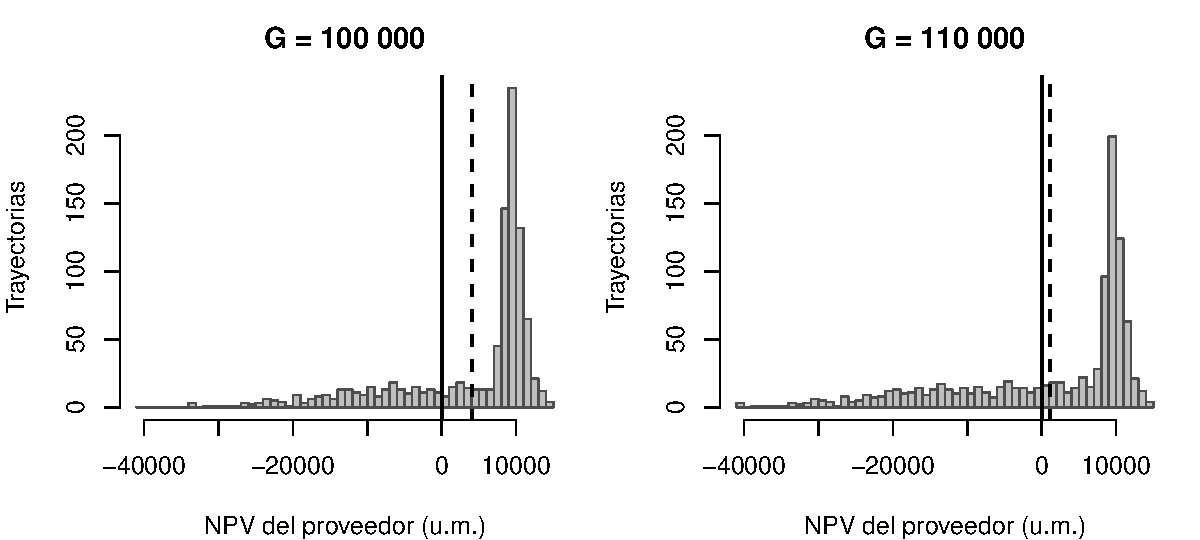
\includegraphics[width=0.85\linewidth]{salidas/figuras/E_histograma_NPV.pdf}
		\caption{NPV del proveedor por trayectoria con la misma escala en ambos paneles. La línea continua marca cero y la discontinua la media.}\label{fig:hist}
	\end{figure}

	Como los cargos no cambian, subir la garantía solo aumenta el complemento: el VP medio del complemento sube 2\,960.94 y el NPV medio baja exactamente lo mismo, de 4\,054.40 a 1\,093.45 (\(-73\,\%\), \cref{tab:garantias}). La garantía de 110\,000 queda muy cerca del saldo mediano al año 5, \(A_0(0.98)^5e^{5m}\approx110\,400\), por eso se activa en casi la mitad de las trayectorias (48.5\,\%). Activación y pérdida no son lo mismo: con \(G=100\,000\) la garantía se activa en el 36.7\,\% de las trayectorias, pero el proveedor pierde solo en el 24.6\,\%, porque los cargos cubren los complementos pequeños; la pérdida aparece cuando el VP del complemento supera el VP de los cargos. En la cola, el CTE\(_{95}\) sube de 22\,959.79 a 29\,892.45 (\(+30\,\%\)) y la \cref{fig:hist} muestra cómo la masa de pérdidas se extiende hacia la izquierda.

	El código comprobó que, con cargo y trayectorias iguales, en ninguna trayectoria la garantía mayor reduce el complemento o aumenta el NPV; en la trayectoria de la \cref{tab:trayres} la diferencia de NPV es \(10\,000\,{}_5p\,v^5=6\,932.66\). Recomendamos \(G=100\,000\): mejor resultado medio y menor pérdida de cola. Estas frecuencias usan la permanencia esperada en cada trayectoria y no simulan eventos demográficos individuales; el VP del complemento con probabilidades reales tampoco es un precio de mercado de la garantía~\cite{Hardy2003}.

	%---------BLOQUE 8------------------- (F: NIIF 17)
	\section{Interpretación conceptual de NIIF 17}\label{sec:F}

	\textbf{1. Flujos y ajuste por riesgo.} En la medición inicial entrarían los flujos dentro del límite del contrato de cinco años: primas futuras, siniestros por fallecimiento, gastos de mantenimiento, comisiones y el gasto de adquisición de 75\,000 por contrato, que es atribuible a la cartera. Serían estimaciones actuales, ponderadas por probabilidad y descontadas con tasas que reflejan las características de los flujos del seguro, no el rendimiento esperado de los activos (el 5\,\% del profit testing no entra)~\cite{NIIF17}. El RA es la compensación que exige la entidad por la incertidumbre no financiera. En este caso es relevante porque el resultado depende mucho de la mortalidad por edad y de la renuncia, y nuestro estrés de renuncia del 6\,\% cambia la cartera en 12\,312 activos al año 5.

	\textbf{2. CSM y contratos onerosos.} La CSM es la utilidad no devengada del grupo, que se reconoce conforme se presta el servicio de cobertura. En un grupo rentable se registra una CSM que evita reconocer ganancia el día uno. En un grupo oneroso no hay CSM: la pérdida se reconoce de inmediato en resultados con un componente de pérdida. Con una prima neta que no cubre el siniestro esperado de ningún año (\cref{tab:brecha}), el grupo de este seguro probablemente sería oneroso, aunque no calculamos FCF, RA ni CSM.

	\textbf{3. NPV positivo no implica CSM positiva.} El profit testing sirve para decidir si lanzar y tarifar el producto: descuenta a la tasa exigida por el accionista (4\,\%), acredita el rendimiento de inversión (5\,\%) y depende de un cuadro de reservas dado, cuyo efecto aquí fue de 97.39 millones. La CSM sale de una medición contable con otras tasas, con un RA que el profit test no incluye y por grupos de contratos: un NPV agregado positivo puede esconder subgrupos onerosos, por ejemplo las edades mayores, donde el siniestro esperado es más alto, y un RA suficientemente grande puede volver negativo el resultado.

	\textbf{4. CSM, reserva y efectivo.} La CSM es una parte del pasivo que representa utilidad futura. La reserva suministrada (40\,000 por contrato al cierre del año 1, 3\,997.13 millones en total) es un supuesto académico que no se construye como FCF más RA más CSM. El efectivo disponible es lo que la aseguradora tiene: 1\,972.52 millones al cierre del año 1 antes de aportes. Que el efectivo no alcance la reserva (\(-2\,024.61\)) es un problema de respaldo y liquidez; que el grupo sea oneroso es un problema de reconocimiento de pérdidas. Por eso liberar reserva no es un cobro y los 3\,050.20 millones de aportes no son utilidad.

	%---------BLOQUE 9------------------- (Contribuciones)
	\clearpage
	\section*{Contribuciones individuales}\label{sec:contribuciones}

	Los tres integrantes participaron en todas las partes del proyecto: programación, revisión cruzada del código y de las cifras, redacción del informe, NIIF 17, nota del foro y presentación. La carga fue equivalente. La tabla indica, para cada integrante, el bloque que coordinó y la verificación que realizó.

	\begin{table}[htbp]
		\centering\small
		\renewcommand{\arraystretch}{1.3}
		\begin{tabularx}{\textwidth}{@{}>{\raggedright}p{3.2cm}>{\raggedright}X>{\raggedright}p{3.0cm}>{\raggedright}p{3.2cm}>{\raggedright\arraybackslash}X@{}}
			\toprule
			\textbf{Integrante} & \textbf{Tarea técnica} & \textbf{Bloque de código} & \textbf{Resultado} & \textbf{Verificación} \\
			\midrule
			Andrey Gonzales (C33329) & Limpieza de la base, decrementos, matriz de transición y varias vidas (A y B); redacción de A y B y apoyo en C--F & \texttt{00\_parametros.R}, \texttt{parteA.R}, \texttt{parteB.R} & \(N_0=104\,004\), proyección a cinco años, matriz y tres rentas de B & Controles de A (Tabla 4) y de B; revisión cruzada de C y E \\
			Randal Picado Bermúdez (C36024) & Profit testing, recursos, escenario adverso y escenario del grupo 2 (C, D y sección 4); redacción de C, D y nota del foro y apoyo en A, B y E & \texttt{parteC-D.R} & NPV, margen, recursos, aportes y comparación de escenarios & Resultado igual a efectivo más reservas; suma de la descomposición del NPV; revisión cruzada de A y B \\
			Anthonny Flores Rojas (C32975) & Equity-linked y NIIF 17 (E y F); redacción de E, F y opinión ejecutiva, presentación y apoyo en A--D & \texttt{parteE.R}, \texttt{main.R} & Simulación, comparación de garantías e integración del informe & Monotonía de garantías y cotejo lognormal analítico; \texttt{main.R} desde cero reproduce las 17 tablas \\
			\bottomrule
		\end{tabularx}
		\caption{Registro de contribuciones por integrante.}\label{tab:contrib}
	\end{table}

	\textbf{Ayudas utilizadas y su comprobación.} Se utilizó inteligencia artificial como apoyo en la escritura de las funciones auxiliares de formato y exportación de tablas (\texttt{fmt} y \texttt{tabla\_tex} en \texttt{00\_parametros.R}), en la limpieza del código y en la redacción y corrección del informe. Los resultados se comprobaron con los controles programados en el código: suma de \(N_0\) por cohortes, probabilidades que suman uno, conservación de activos, proyección matricial frente a directa, resultado económico igual a efectivo más efecto de reservas, suma de la descomposición del NPV y monotonía de las dos garantías en cada trayectoria. Las frecuencias de activación de la \cref{sec:E} también se cotejaron con la probabilidad lognormal analítica (38.4\,\% y 49.6\,\%, frente a 36.7\,\% y 48.5\,\% simulados).

	\textbf{Reproducibilidad.} Instalar \texttt{readxl}, abrir \texttt{Contingencias-II.Rproj} y ejecutar \texttt{source("Codigo/main.R")}. Las tablas quedan en \texttt{Informe/salidas/tablas}, la figura en \texttt{Informe/salidas/figuras} y el detalle por cohorte y por trayectoria en \texttt{Informe/salidas/resultados}.

	%---------BLOQUE 10------------------- (Bibliografia)
	\begin{thebibliography}{9}\small

		\bibitem{Guia2026}
		Y. Ramírez Morera, ``Proyecto final: guía del grupo 2,'' CA-0309 Contingencias de Vida II, Escuela de Matemática, Universidad de Costa Rica, II ciclo 2026.

		\bibitem{Dickson2020}
		D. C. M. Dickson, M. R. Hardy, H. R. Waters, \emph{Actuarial Mathematics for Life Contingent Risks}, 3.\textsuperscript{a} ed., Cambridge University Press, 2020.

		\bibitem{Hardy2003}
		M. R. Hardy, \emph{Investment Guarantees: Modeling and Risk Management for Equity-Linked Life Insurance}, John Wiley \& Sons, 2003.

		\bibitem{NIIF17}
		International Accounting Standards Board, \emph{NIIF 17 Contratos de Seguro}, IFRS Foundation, 2017 (modificada en 2020).

	\end{thebibliography}

	%---------BLOQUE 11------------------- (Anexos)
	\clearpage
	\section*{Anexos}\label{sec:anexos}

	\subsection*{Anexo E. Detalle de una trayectoria}

	Se toma la primera trayectoria (número 4) en que la garantía se activa con ambos valores. Con estas filas se verifican la cuenta \eqref{eq:cuenta}, los cargos, el complemento y el NPV \eqref{eq:npvE} de las dos garantías.

	\begin{table}[htbp]
		\centering\small
		\tabla{E_trayectoria_detalle}
		\caption{Trayectoria 4: choques, saldo de la cuenta, cargos y su valor presente ponderado por permanencia, en \um}\label{tab:tray}
	\end{table}

	\begin{table}[htbp]
		\centering\small
		\tabla{E_trayectoria_detalle_resumen}
		\caption{Trayectoria 4: complemento al vencimiento y NPV con ambas garantías, en \um}\label{tab:trayres}
	\end{table}

	\subsection*{Archivos de detalle}

	El detalle completo está en \texttt{Informe/salidas/resultados} (CSV con separador punto y coma): proyección por cohorte de edad y sexo (\texttt{A\_proyeccion.csv}), probabilidades y rentas por pareja (\texttt{B\_probabilidades.csv}, \texttt{B\_rentas\_por\_cohorte.csv}), flujos y recursos de los tres escenarios (\texttt{C\_}, \texttt{D\_} y \texttt{S4\_}) y las 1\,000 trayectorias con sus choques y NPV (\texttt{E\_simulacion.csv}).

\end{document}
